\subsection{Textual Syntax}
\begin{figure}[h]
	\centering 
	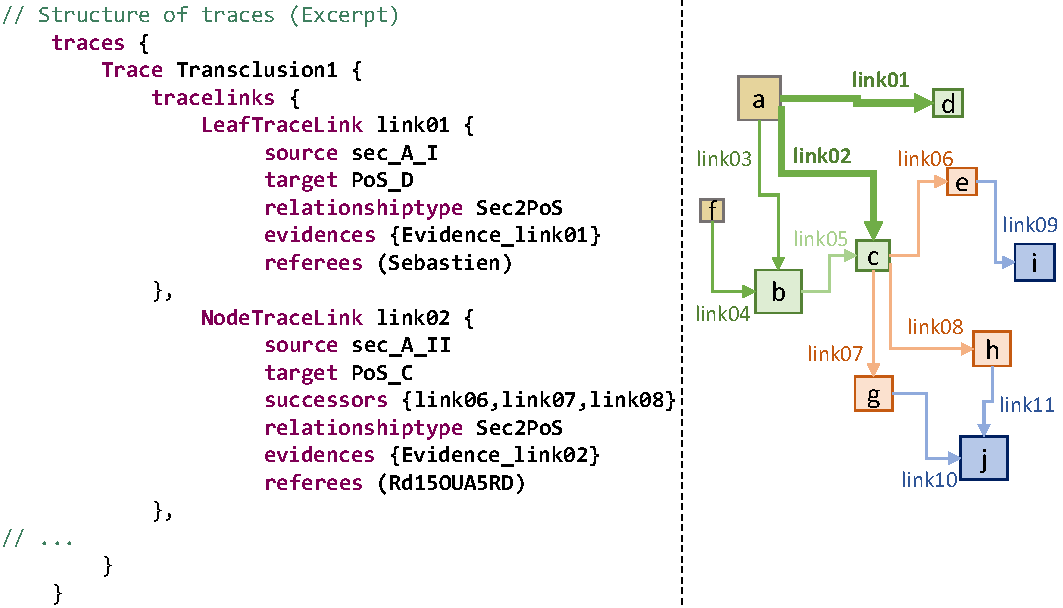
\includegraphics[width=.95\linewidth]{images/listing-struct.pdf}
	\caption{Textual syntax excerpt: core structure of a trace.}
	\label{fig:textualsyntax-struct}
\end{figure}
We chose to use a JSon-like grammar as a first generic textual syntax of Tracea. We believe this type of concrete syntax is appropriate. It is verbose, but \textit{i)} it is readable by humans without holding any structural information from the abstract syntax, and \textit{ii)} known generators can be easily adapted to generate instances. The complete grammar definition has been uploaded on the Modelia Git repository~\cite{Tracea_Repo}.

As can be seen in the excerpt parts of Figure \ref{fig:textualsyntax-struct}, \ref{fig:textualsyntax-declare}, and \ref{fig:textualsyntax-integrity}, classes and structural features of the metamodel are keywords of the grammar. Qualified named are used to navigate into inner elements (\textit{i.e.,} following the pattern \verb|'Root.element.innerElement'| structure with the dot as connector). Elements of a list are set between brackets \verb|{}| and separated with a coma \verb|,|.

\begin{figure}[h]
	\centering 
	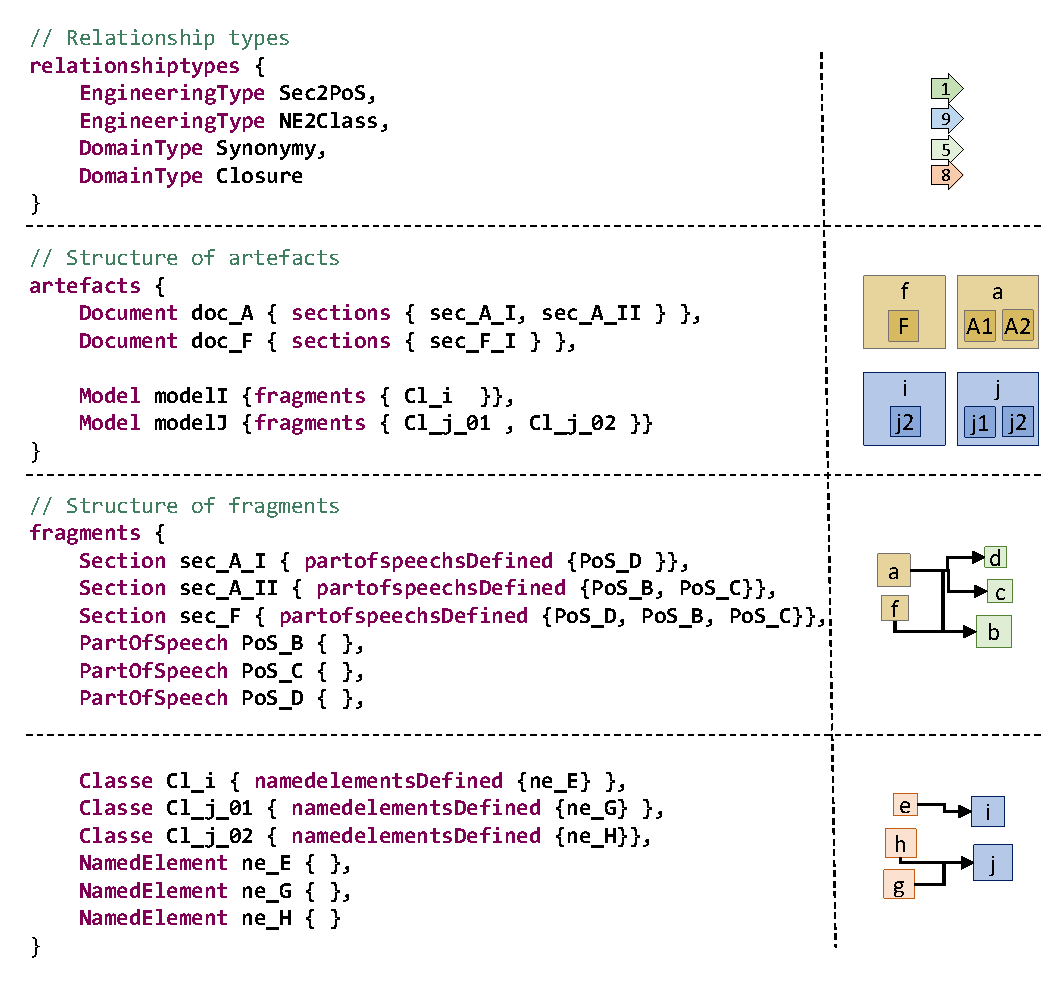
\includegraphics[width=.9\linewidth]{images/listing-art-n-types.pdf}
	\caption{Textual syntax excerpt: artefacts, fragments, and types declarations.}
	\label{fig:textualsyntax-declare}
\end{figure}
In Figure \ref{fig:textualsyntax-struct} \texttt{Traces} are declared sequentially. They contain the declaration of their \texttt{TraceLinks}. Figure \ref{fig:textualsyntax-declare} shows examples of \texttt{RelationshipTypes} declarations, and \texttt{Artefacts} and \texttt{Fragments} decomposition. These elements can be later referenced in different elements of the system. Their dependence level to other elements is weak. In the same manner, Figure \ref{fig:textualsyntax-integrity} presents two \texttt{Evidences} declarations and two \texttt{Referees}.

\begin{figure}[h]
	\centering 
	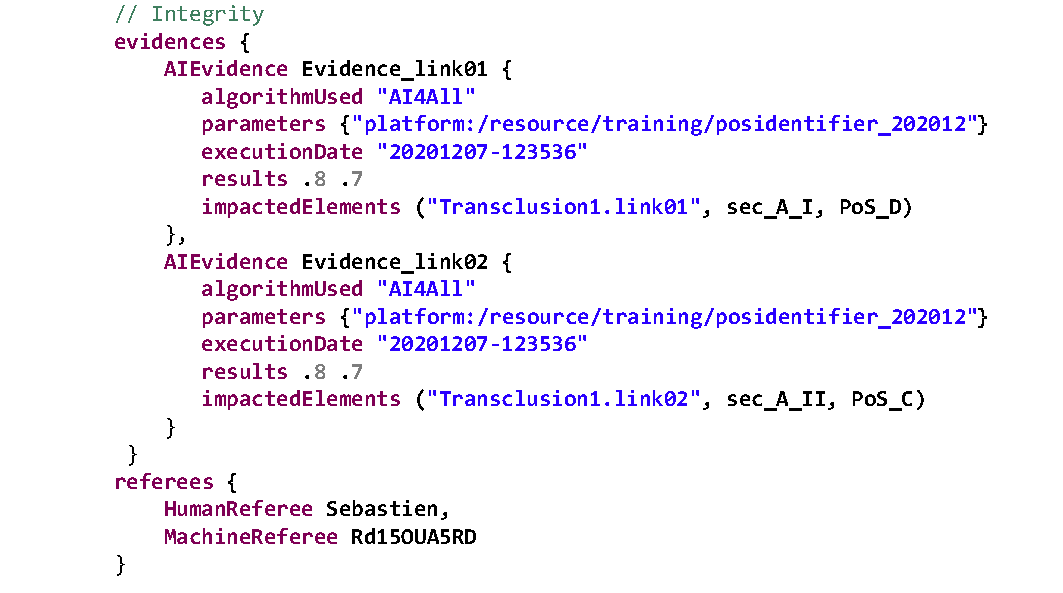
\includegraphics[width=.9\linewidth]{images/listing-integrity.pdf}
	\caption{Textual syntax excerpt: integrity elements declarations.}
	\label{fig:textualsyntax-integrity}
\end{figure}
